\epigraph{For neural machine translation, it all started from language
modeling.}{Thang Luong.}

Language modeling plays an
indispensable role in ensuring that machine translation systems produce fluent target
sentences and has always been an active area of research.
Despite much effort in improving traditional \ngram{} language models
\cite{rosenfeld2000,srilm,teh2006,irstlm,kenlm,pauls2011,heafield13},
traditional LMs inherently can only handle short
contexts of a few words. Approaches to building \nlmtext{} (\nlms) using
feed-forward networks such as those initiated by \newcite{Bengio2003} and
enhanced by others \cite{Morin2005,Bengio08,MnihHinton2009,MnihTeh2012} have %,Mnih2007
addressed that drawback to model longer contexts.
% worked great compared to traditional \ngram{} language models. 
Still, \nlms{} can only capture fixed-length contexts and is
incapable of handling variable-length sequences, which is the case for sentences.
Recurrent neural networks (RNNs) come in handy as a powerful and expressive
architecture to handle sequential data and have successfully been applied to the
language modeling task \cite{MikolovKBCK10,MikolovKBCK11,mikolovLM}.
By viewing RNNs as generative models \cite{Sutskever11} that can produce texts 
and by pushing another step towards conditioning RNNs on source sentences, recent works
\cite{kal13,sutskever14,cho14} have started a new line of resesarch in machine translation, namely Neural
Machine Translation (NMT). NMT is technically a source-conditioned \nlm{} that
can be trained end-to-end.

%Early success of feed-forward \nlms{} has led to widespread adoption of \nlms{}
%as an additional component in the machine translation pipeline
%such as \cite{schwenk07,vaswani13decode,luong15nlm}, inter alia.
%\cite{Schwenk12continuous,Son:2012:CST,Auli13,devlin14}

%An important part in the machine translation pipeline is the ability to model language
%coherence at the target side. 
%As such, a significant amount of effort in
%improving MT has centered around enhancing language modeling -- more specifically, the need to capture long-range
%dependencies better. We start out with efforts to scale up traditional \ngram{} language models 

In this chapter, we provide background knowledge on two main topics, RNN and NMT.
We first go through the basics of RNNs, explaining how they can be used to model sentences. 
Then, we delve into details of one particular type of RNNs, the Long Short-term Memory, that makes training RNNs easier.
Given RNNs as a building block, we discuss NMT together with tips and tricks for better training and testing NMT.

\section{Recurrent Neural Network}
Recurrent Neural Network (RNNs) \cite{elman90} are models that help understand
the temporal aspect as well as build up representations for sequential data
using a dynamic memory structure. At the surface form, an RNN takes as input a sequence of vectors $\x{1},
\x{2}, \ldots, \x{n} \inR{d}$ and processes them one by one. For each
new input $\x{i}$, an RNN updates its memory to produce a hidden state
$\hid{i}$ which one can think of as a representation for the partial sequence
$\x{\overline{1,i}}$. %$\x{1},\ldots, \x{i}$. 
The beauty of RNNs lies in the fact that it can
capture the dynamics of an arbitrarily long sequence without having to increase its modeling
capacity unlike the case of feedforward network which can only model
relationship within a fixed-length sequence. The key secret sauce is in the
recurrence formula of an RNN that defines how its hidden state is updated. At
its simplest form, a ``vanilla'' RNN defines its recurrence function as:
\begin{align}
\MB{h}_t &= f\paren{\x{t}, \hid{t-1}} \label{e:abstract_rnn} \\
&= \sigma \paren{\W{xh}\x{t} + \W{hh}\hid{t-1}} \label{e:vanilla_rnn}
\end{align}
In the above formula, $f$ is an abstract function that computes a new hidden state given the current input $\x{t}$ and the
previous hidden state $\hid{t-1}$. We provide in \eq{e:vanilla_rnn} one popular choice
of $f$ with $\sigma$ being a non-linear function such as $\sigmoid$ or $\tanh$.
At each timestep $t$, an RNN can (optionally) emit an output symbol
$y_t$ which can either be discrete or real-valued. For the discrete scenario,
which is often the case for languages, a probability distribution $\bm{p}$ over a 
set of output classes $Y$ is derived as
follows\footnote{For the real-valued case, we refer readers to mixture density
models \cite{bishop94} which have been applied to RNN training, e.g., for
hand-writing synthesis \cite{graves13c}.}:
\begin{align}
\bm{s} &= \W{hy}\hid{t} \label{e:score} \\
\bm{p} &= \softmax(\bm{s}) \label{e:prob}
\end{align}
Here, we introduce a new set of weights $\W{hy} \inR{|Y| \times d}$, with $d$ being the dimension of the RNN hidden
state, to compute a score vector $\bm{s}$, or {\it logits}, over
different individual classes. Often, with a large output set $Y$, the
matrix-vector multiplication in \eq{e:score} is a major computational
bottleneck in RNNs, which results in several challenges for neural language modeling
and machine translation that we will mention later. 

The $\softmax$ function transforms the score
vector $\bm{s}$ into a vector of probability $\bm{p}$, which is defined for each specific
element $y \in Y$ as below.
For convenience, we overload our notations to use $p(y)$ and $s(y)$ to refer to entries in
the vectors $\bm{p}$ and $\bm{s}$ that correspond to $y$.
\begin{align}
p(y) = \frac{\e^{s(y)}}{\sum_{y' \in Y} \e^{s(y')}}
\label{e:softmax}
\end{align}

With the above formulae, we have completely defined the RNN weight set $\theta\!=\!\{\W{xh},
\W{hh}, \W{hy}\}$, which consists of {\it input} connections $\W{xh}$, {\it
recurrent} connections $\W{hh}$, and {\it output}
connections $\W{hy}$. These weights are shared across
timesteps as illustrated in Figure~\ref{f:rnn} \error{Draw a picture on
general RNNs}, which enables
RNNs to handle arbitrarily long sequences.

\begin{figure}[tbh!]
\centering
%\psgrid
\rput(7.1,2.6){{\color{lightblue} $\MB{W_{hh}}$}}
\rput(8.6,1.0){{\color{lightgreen} $\MB{W_{xh}}$}}
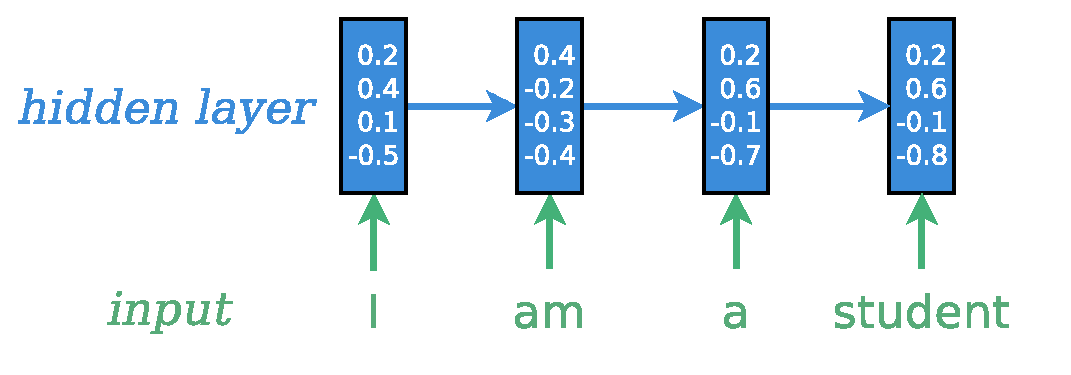
\includegraphics[width=0.6\textwidth, clip=true, trim= 0 0 0 0]{img/rnn.eps} % , angle=-90
\caption[Recurrent neural networks]{{\bf Recurrent neural networks} -- example of a recurrent
neural network that processes a sequence of input words \word{I am a student} to
build up hidden representations as input symbols are consumed. The recurrent
$\MB{W_{hh}}$ and feed-forward $\MB{W_{xh}}$ weights are shared across
timesteps.
} 
\label{f:rnn}
\end{figure}

Next, we discuss the training and testing phases of RNNs from a slightly more
focused angle, the language learning aspect. For more details on RNNs, we refer readers to the following resources
\cite{sutskever12,mikolov12,karpathy15rnn}.

\subsection{Recurrent Language Models}
To apply RNNs to sentences in languages, or generally sequences of discrete symbols, one can
consider one-hot representations $\x{i} \inR{|V|}$, with $V$ being the
vocabulary considered. However, for a large
vocabulary $V$, such a representation choice is problematic as it results in
a large weight matrix $\W{xh}$ and there is no notion of similarity between
words. In practice, low-dimensional dense representations for words, or {\it
word embeddings}, are often used to address these problems. Specifically, an
embedding matrix
$\W{e} \inR{d \times |V|}$ is looked up for each word $x_i$ to retrieve a
representation $\x{i} \inR{d}$. As a result, a simple RNN applied to language
modeling will generally have $\theta = \{\W{xh}, \W{hh}, \W{hy}, \W{e}\}$ as its
weights as illustrated in Figure~\ref{f:rlm} \error{Draw an RNN with
embedding}.

In language modeling (LM), the task is to specify a probability distribution over
sequences of symbols (often, words) so that one can judge if a sequence of
words is more likely or ``fluent'' than another. To accomplish that, an LM decomposes the
probability of a word sequence $y = y_1, \ldots,
y_m$ as:
\begin{align}
p(y) = \prod_{i=1}^m p(y_i | y_{<i}) %\yrange{1}{i-1})
\end{align}
In the above formula, each of the
individual term $p(y_i | y_{<i})$ is the conditional probability of the current
word $y_i$ given previous words $y_{<i}$, also referred as the {\it
context} or the {\it history}. To model these conditional probabilities, traditional \ngram{}
as well as feedforward-based neural language models have to resort to the
Markovian assumption to model only a fixed window of context, i.e., $p(y_i |
y_{i-n+1}, \ldots, y_{i-1})$. An RNN-based language model naturally lends itself to model the full
history as we shall see now.

An RNN-based language model (RNNLM) is a special case of RNNs in which: (a) the input and output
are sequences of discrete words, (b) the output sequence ends %$y=\{y_1, \ldots, y_n$, \eos$\}$ 
with a special symbol \eos{} that marks the boundary, e.g., $y=\{$ ``I'', ``am'', ``a'',
``student'', \eos$\}$, and (c) the input sequence is a
shift-by-1 version of the output sequence with \sos{} as a starting symbol,
e.g., $x=\{$ \sos, ``I'', ``am'', ``a'',
``student''$\}$. We illustrate this in \figref{f:rlm}.

%i.e., $x=\{$
%\sos{}, $y_1, \dots, y_n\}$. In our example, $x=\{$ \sos, ``I'', ``am'', ``a'',
%``student''$\}$, whereas $y=\{$ ``I'', ``am'', ``a'',
%``student'', \eos$\}$
\paragraph{Training}
Given a training dataset of $N$ discrete output sequences $\ytop{1}, \ldots,
\ytop{N}$ with lengths $m_1, \ldots, m_N$ accordingly. The learning objective is
to minimize the negative log-likelihood, or the {\it cross-entropy} loss, of these training examples:
\begin{align}
J(\thetav) &= \sum_{i=1}^{N} -\log p\paren{\ytop{i}} \\ 
&= \sum_{i=1}^{N} \sum_{t=1}^{m_i} -\log p\paren{\ytop{i}_t |
\ytop{i}_{<t}}
\end{align}

RNN learning is often done using mini-batch stochastic gradient descent (SGD) algorithms in
which a small set of training examples, a {\it mini-batch}, is used to compute
the gradients and update weights one at a time. Using mini-batches has
several advantages: (a) the gradients are more reliable and consistent than the
``online'' setting which updates per example, (b) less computation is required to
update the weights unlike the case of full-batch learning which has to process
all examples before updating, and (c) with multiple examples in a mini-batch,
one can turn matrix-vector multiplications such
as those in \eq{e:vanilla_rnn} and \eq{e:score} into matrix-matrix multiplications which can be
deployed efficiently on GPUs. The simplest weight update formula with $\eta$ as
a learning rate is given below:
\begin{align}
\thetav \longleftarrow \thetav - \eta \grad{J(\thetav)} %\fracder{J(\thetav)}{\thetav}
\end{align}

\paragraph{Backpropagation} To compute the gradients for the loss $J(\thetav)$,
we first need to compute the derivative of predicting $y_t$ at timestep $t$. We
will now work out the gradients with respect to $\W{hy}$ and $\hid{t}$, i.e., up
to \eq{e:score}. The remaining derivations will depend on the choice of the RNN
hidden unit $f$ defined in \eq{e:abstract_rnn}.
\begin{align*}
\fracder{\log p(y_t)}{\thetav} &= \parfrac{\thetav} \paren{s(y_t) - \log \sum_{y'}
e^{s(y')}} && \text{[From \eq{e:softmax}]} \\
&= \fracder{\bm{s}}{\thetav} \cdot \parfrac{\bm{s}} \paren{s(y_t) - \log \sum_{y'}
e^{s(y')}} && \text{[Chain rule in vector calculus]} \\
\end{align*}

Computing per-coordinate gradient, we have:
\begin{align}
 \parfrac{s(y)} \paren{s(y_t) - \log \sum_{y'} e^{s(y')}} =
  \begin{cases}
   1 - p(y_t) & y = y_t \\
   -p(y) & y \neq y_t
  \end{cases}
\end{align}
Here, $\bm{p}$ is the probability distribution defined in \eq{e:prob} and the
above gradients can be concisely written in vector form as $\bm{1}_{y_t} -
\bm{p}$. We should note that $\bm{p}$ has been calculated in the forward pass,
so we simply reuse it. $\bm{1}_{y_t}$ is a one-hot vector with 1 at position
$y_t$. Combining the above formulae, we simplify:
\begin{align}
\fracder{\log p(y_t)}{\thetav} &= \fracder{\bm{s}}{\thetav} \cdot (\bm{1}_{y_t}
- \bm{p})
\end{align}

With respect to $\W{hy}$, we have:

With respect to $\hid{t}$, we have:
\begin{align}
\fracder{\log p(y_t)}{\hid{t}} &= \fracder{\bm{s}}{\hid{t}} \cdot (\bm{1}_{y_t}
- \bm{p}) \\
 &= \fracder{\W{hy}\hid{t}}{\hid{t}} \cdot (\bm{1}_{y_t} - \bm{p}) \\
 &= \bm{W}^{\top}_{hy}(\bm{1}_{y_t} - \bm{p})
\end{align}


\error{Write derivative lemma}

\begin{figure}[tbh!]
\centering
%\psgrid
\rput(7.1,2.6){{\color{lightblue} $\MB{W_{hh}}$}}
\rput(8.6,1.0){{\color{lightgreen} $\MB{W_{xh}}$}}
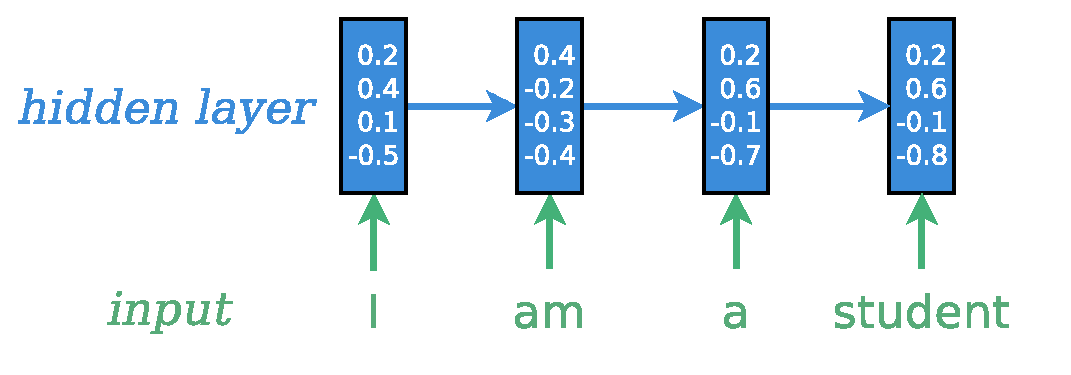
\includegraphics[width=0.6\textwidth, clip=true, trim= 0 0 0 0]{img/rnn.eps} % , angle=-90
\caption[Recurrent language models]{{\bf Recurrent language models} -- example of a recurrent
neural network that processes a sequence of input words \word{I am a student} to
build up hidden representations as input symbols are consumed. The recurrent
$\MB{W_{hh}}$ and feed-forward $\MB{W_{xh}}$ weights are shared across
timesteps.
} 
\label{f:rlm}
\end{figure}

For simplicity and convenience, one can set the embedding size to be equal to the
hidden size, so $\W{xh}, \W{hh} \inR{d \times d}$. We can further simplify the
notation to have $\rnn = [\MB{W_{xh}} \MB{W_{hh}}]$, so \eq{e:vanilla_rnn}
becomes:
\begin{align}
\MB{h_t} = \sigma \paren{\rnn
\begin{bmatrix}
  \MB{x_t} \\
  \MB{h_{t-1}}
 \end{bmatrix}
}
\end{align}


\subsection{Better Training RNNs}
\paragraph{Vanishing Gradient Problem}

\cite{pascanu13}

\begin{align}
\MB{h}_t = \sigma \paren{
\MB{W_{xh}}\MB{x}_t + \MB{W_{hh}}\MB{h}_{t-1}
}
\end{align}

\begin{align}
\fracder{\MB{h}_t}{\MB{h}_{t-1}} = \diag\paren{\sigma'(\ldots)}\tp{\MB{W_{hh}}}
\end{align}

\begin{align}
\norm{\fracder{\MB{h}_t}{\MB{h}_{t-1}}} & \leq \norm{\diag\paren{\sigma'(\ldots)}} 
\norm{\tp{\MB{W_{hh}}}} \\ 
& \leq \gamma \lambda_1
\end{align}

\begin{align}
\norm{\fracder{\MB{h}_t}{\MB{h}_{t-k}}} \leq \paren{\gamma \lambda_1}^{k}
\rightarrow 0 & \quad \text{ if } \lambda_1 < \frac{1}{\gamma}
\end{align}

\begin{align}
\fracder{\MB{c}_t}{\MB{c}_{t-1}} = \MB{I}
\end{align}

\paragraph{Long Short-Term Memory}
We use the formulation of \cite{zaremba14}.
For a single LSTM block at layer $l$ and time $t$, the new hidden state $\hlt$ and memory cell $\clt$ are calculated from $\MB{h_t^{l-1}}$, $\MB{h_{t-1}^l}$ and $\MB{c_{t-1}^l}$ like so:
\begin{align}
\label{eqn:LSTMdef1}
\begin{pmatrix}
\ilt \\
\flt \\
\olt \\
\glt
\end{pmatrix}
&= 
\begin{pmatrix}
\sigm \\
\sigm \\
\sigm \\
\tanh
\end{pmatrix}
\MB{T}_{4n \times 2n}
\begin{bmatrix}
  \MB{h_t^{l-1}} \\
  \MB{h_{t-1}^l}
 \end{bmatrix} \\
\clt &= \flt \circ \MB{c_{t-1}^l} + \ilt \circ \glt \\
\hlt &= \olt \circ \tanh(\clt)
\end{align}
where $\sigm$ and $\tanh$ are applied element-wise, $\circ$ denotes element-wise multiplication, 
and $\MB{T}_{4n \times 2n}$ is a $4n \times 2n$ matrix of weights that depends on $l$ but not $t$.\footnote{Note: Sometimes these equations are written omitting the superscript $l$ and writing $\MB{h_t^{l-1}}$ as $x_t$, but for the purposes of deriving the back-propagation equations, we need to refer to the layer $l$ explicitly.}
If $l=1$ then $\MB{h_t^{l-1}}$ is the input vector $x_t$.
If $t=1$ then $\MB{h_{t-1}^l}$ and $\MB{c_{t-1}^l}$ are taken to be zero.

An LSTM block at layer $l \in \{1, \dots L\}$ and time $t \in \{1, \dots T\}$ consists of:
\begin{itemize}
\item The hidden state $\hlt \in \mathbb{R}^n$
\item The memory cell $\clt \in \mathbb{R}^n$
\item The input gate $\ilt \in [0,1]^n$
\item The forget gate $\flt \in [0,1]^n$
\item The output gate $\olt \in [0,1]^n$
\item The input modulation gate $\glt \in [0,1]^n$
\end{itemize}
We call $n$ the LSTM block size.

\subsection{LSTM Backpropation}
$\MB{\delta_{c^{(2)}}}$

$\MB{\delta_{h^{(2)}}}$

$\MB{\delta_{c^{(1)}}}$

$\MB{\delta_{h^{(1)}}}$

$\MB{\delta_{c}} \pluseq \MB{\delta_{h}}\MB{o_t}\tanh'(\MB{c_t}) $

$\MB{\delta_{c}} = \MB{\delta_{c}} \circ \MB{f_t} $

$\MB{\delta_{h}} \pluseq \text{upper grad}$


\section{Neural Machine Translation}
\begin{figure}[tbh!]
\centering
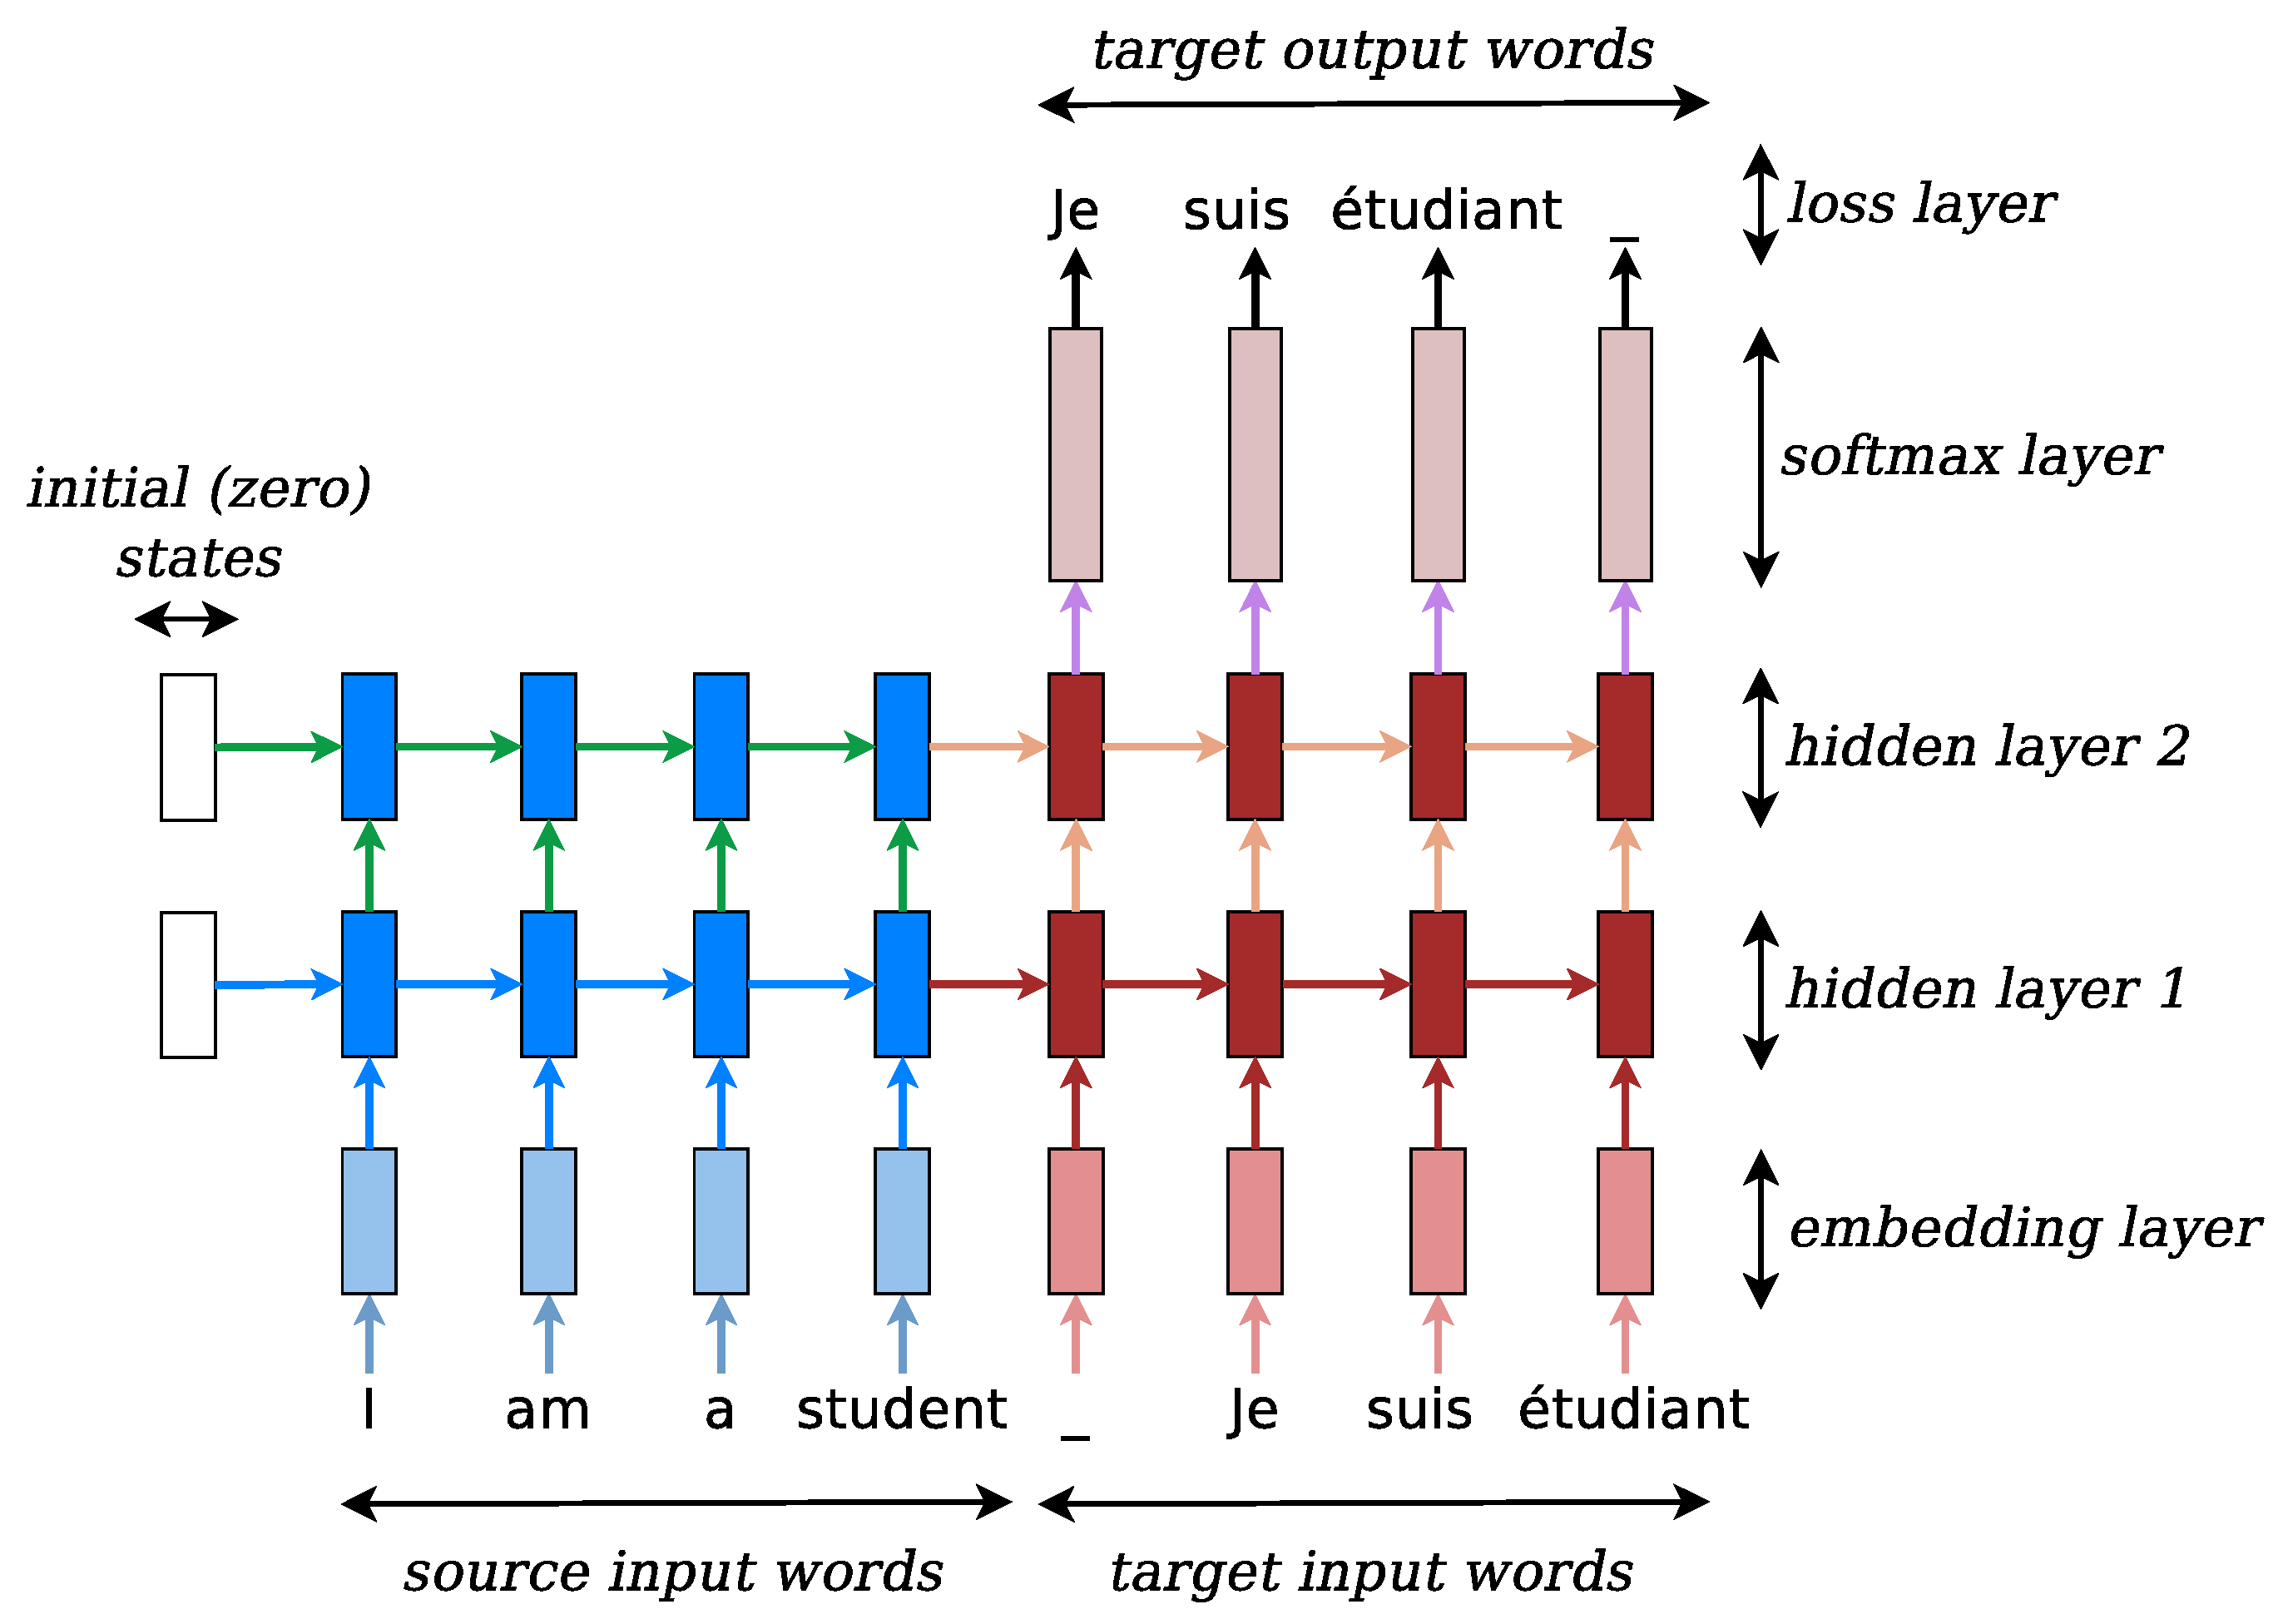
\includegraphics[width=0.8\textwidth, clip=true, trim= 0 0 0
0]{img/nmt_very_details.eps} % , angle=-90
\caption[Neural machine translation]{{\bf Neural machine translation} -- example of a deep recurrent
architecture proposed by \newcite{sutskever14} for
translating a source sentence \word{I am a student} into a target sentence
\word{Je suis \'{e}tudiant}. Here, \word{\texttt{\_}} marks the end of a sentence.
} 
\label{f:nmt_details}
\end{figure}


Neural machine translation aims to directly model the conditional probability $p(\tgt{}|\src{})$ of translating
a source sentence, $\src{1},\ldots,\src{n}$, to a target sentence, $\tgt{1},\ldots,\tgt{m}$.
It accomplishes such goal through the {\it encoder-decoder} framework \cite{sutskever14,cho14}. The {\it encoder} computes a representation $\MB{s}$
for each source sentence. Based on that source representation,
the {\it decoder} generates a translation, one target word at a time, and hence, decomposes the conditional probability as:
\begin{equation}
\log p(\tgt{}|\src{}) = \sum_{j=1}^m \nolimits \log
p\paren{\tgt{j}|\tgt{<j},\src{},\MB{s}}
\end{equation}

A natural choice to model such a decomposition in the decoder is to use a
recurrent neural network (RNN) architecture, which most of the recent NMT work have in common. They,
however, differ in terms of the RNN architectures used and how the encoder computes the source representation $\MB{s}$.
%, e.g., vanilla RNN, long-short term memory (LSTM) \cite{lstm97} or gated recurrent units \cite{cho14}

Kalchbrenner and Blunsom \cite{kal13} used an RNN with the vanilla RNN unit for the decoder and a
convolutional neural network for encoding the source. On
the other hand, Sutskever et al. \cite{sutskever14} and Luong et al.
\cite{luong15,luong15attn} built deep RNNs with the Long Short-Term Memory (LSTM) unit
\cite{lstm97} for both the encoder and the decoder. Cho et al., \cite{cho14}, Bahdanau et al.,
\cite{bog15}, and Jean et al. \cite{jean15,mono15} all adopted an
LSTM-inspired hidden unit, the gated recurrent unit (GRU), and used bidirectional
RNNs for the encoder.
%\footnote{They all used a single RNN layer except for the latter two
%works which utilized a bidirectional RNN for the encoder.}

In more details, considering the top recurrent layer in a deep RNN architecture, one can compute the probability of decoding each target word $y_j$ as:
\begin{equation}
p\left(\tgt{j}|\tgt{<j},\src{},\MB{s}\right) = \softmax\paren{\hd{j}}
\end{equation}
%with $g$ being the transformation function that outputs a vocabulary-sized
%vector.\footnote{One can provide $g$ with other inputs such as the currently
%predicted word $\tgt{j}$ as in \cite{bog15}.} 
with $\hd{j}$ being the current target hidden state computed as:
\begin{equation}
\label{e:rnn}
\hd{j} = f(\hd{j-1}, \tgt{j-1}, \MB{s})
\end{equation}
Here, $f$ derives the current state given the previous state
$\hd{j-1}$, the
current input (often the previous word $\tgt{t-1}$), and optionally, the source
representation $\MB{s}$.
$f$ can be a vanilla RNN unit, a GRU, or an LSTM. 
The early NMT approach  \cite{kal13,sutskever14,cho14,luong15} uses the last source hidden state
$\MB{s}=\hb{n}$ once to initialize the decoder hidden state and sets $\MB{s}=[\text{ }]$ in
\eq{e:rnn}.

\subsection{Training}
The training objective is formulated as follows:
\begin{equation}
J = \sum_{(\src{},\tgt{}) \in \mathbb{D}} \nolimits -\log p(\tgt{}|\src{})
\label{e:j_t}
\end{equation}
with $\mathbb{D}$ being our parallel training corpus.

mention bucketing and batching

\subsection{Testing}

mention beam-search, ensemble

\begin{figure}[tbh!]
\centering
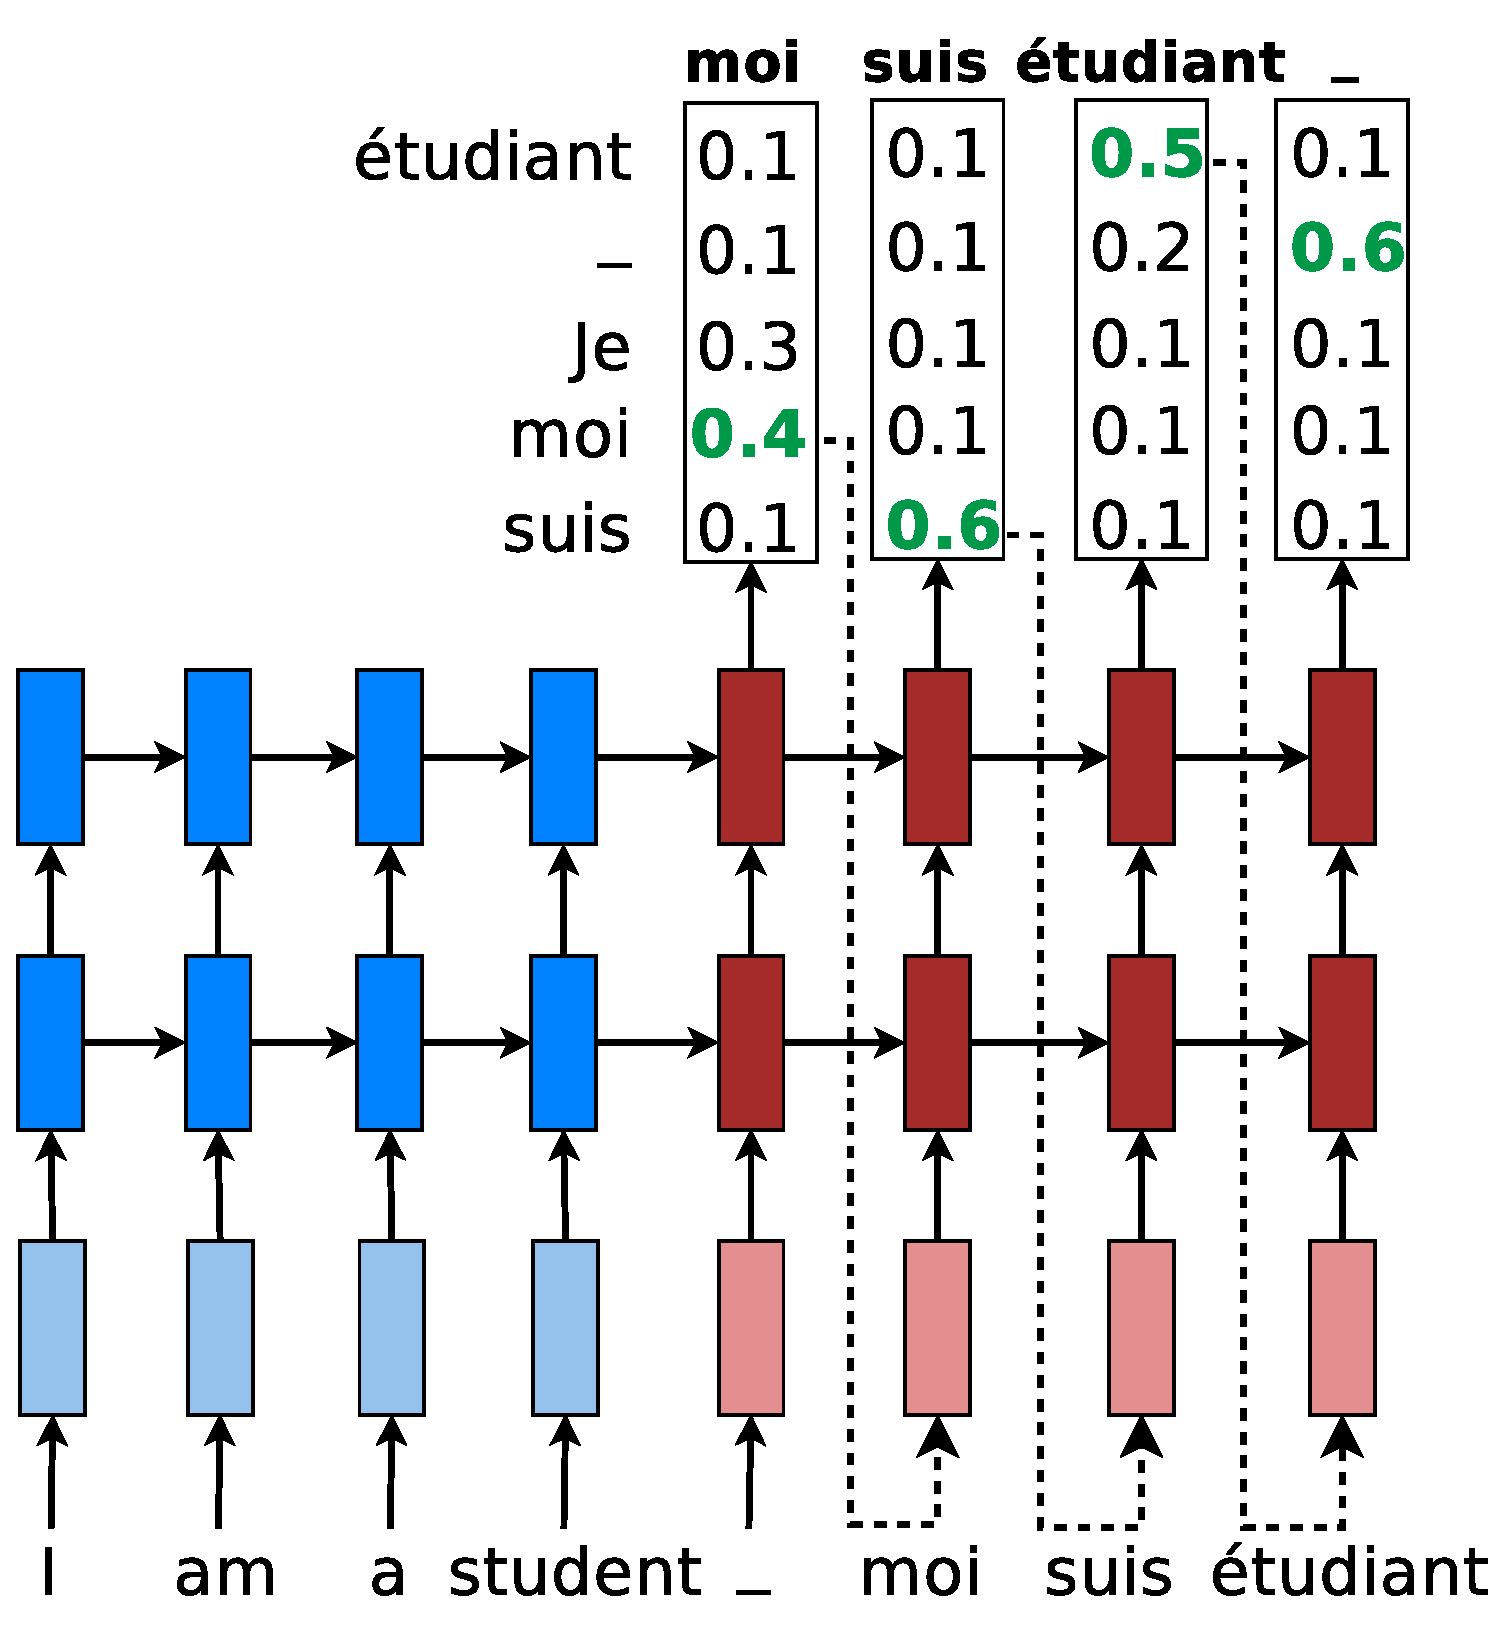
\includegraphics[width=0.6\textwidth, clip=true, trim= 0 0 0
0]{img/nmt_test.eps} % , angle=-90
\caption[Neural machine translation]{{\bf Neural machine translation} -- example of a deep recurrent
architecture proposed by \newcite{sutskever14} for
translating a source sentence \word{I am a student} into a target sentence
\word{Je suis \'{e}tudiant}. Here, \word{\texttt{\_}} marks the end of a sentence.
} 
\label{f:nmt_details}
\end{figure}


%\section{Backward Propagation}
%\subsection{Definitions}
In this section we define some additional notation that will help us to derive the necessary back-propagation equations.

\begin{definition}
Let $U$ and $V$ refer to the $n \times n$ weight matrices corresponding to the following portions of $\MB{T}_{4n \times 2n}$:
\begin{equation}
\MB{T}_{4n \times 2n} = 
\begin{bmatrix}
U_i & V_i \\
U_f  & V_f\\
U_o & V_o\\
U_{\hat{h}} & V_{\hat{h}} \\
\end{bmatrix}
\end{equation}
In particular, we will use the superscript $l$ to denote these matrices used to calculate layer $l$ in Equation (\ref{eqn:LSTMdef1}).
\end{definition}

\begin{definition}
\label{def:z}
For all $l \in \{1,\dots,L\}$ and $t \in \{1,\dots,T\}$, define the \emph{weighted inputs}
\begin{alignat*}{2}
&\zilt = U_i \MB{h_t^{l-1}} + V_i \MB{h_{t-1}^l} \hspace{50pt}
&\zflt = U_f \MB{h_t^{l-1}} + V_f \MB{h_{t-1}^l}\\
&\zolt = U_o \MB{h_t^{l-1}} + V_o \MB{h_{t-1}^l} 
&\zglt = U_{\hat{h}} \MB{h_t^{l-1}} + V_{\hat{h}} \MB{h_{t-1}^l}
\end{alignat*}
so that 
\begin{equation}
\begin{pmatrix}
\ilt \\
\flt \\
\olt \\
\glt
\end{pmatrix}
=
\begin{pmatrix}
\sigm \\
\sigm \\
\sigm \\
\tanh
\end{pmatrix}
\begin{pmatrix}
\zilt \\
\zflt \\
\zolt \\
\zglt
\end{pmatrix}
\end{equation}
where $\sigm$ and $\tanh$ are applied element-wise.
We call $\zilt$ the \emph{weighted input} to the input gate $\ilt$.
\end{definition}

\begin{definition}
Define the \emph{error} of the input, forget, output and input modulation gates at layer $l$ and time $t$ to be
\begin{alignat*}{2}
\dilt &= \fracder{L}{\zilt} \hspace{50pt}
\dflt &&= \fracder{L}{\zflt} \\
\dolt &= \fracder{L}{\zolt} \hspace{50pt}
\dglt &&= \fracder{L}{\zglt} 
\end{alignat*}
where $L$ is the loss function. Note: $\dilt$ is the partial derivative of $L$ with respect to the weighted input $\zilt$, \emph{not} $\ilt$.
\end{definition}

\begin{definition}
Define the \emph{error} of the hidden state and cell and layer $l$ and time $t$ to be
\begin{align}
\dhlt = \fracder{L}{\hlt} \hspace{50pt} \dclt = \fracder{L}{\clt}
\end{align}
where $L$ is the loss function.
\end{definition}

\subsection{Derivations}
In this section we will derive expressions for $\dhlt$, $\dclt$, $\dilt$, $\dflt$, $\dolt$, and $\dglt$ in terms of the $\MB{\delta}$ values for the $(l+1,t)$ and $(l,t+1)$ blocks. 
These expressions will enable us to do back-propagation through time and layers.
If you are not interested in the derivations, skip ahead to Section \ref{subsec:summary} to see the final back-propagation equations.
\begin{lemma}
For $l \in \{1,\dots, L-1\}$ and $t \in \{1, \dots, T-1\}$,
\begin{equation}
\dhlt = 
\begin{bmatrix}
U_i^\top & U_f^\top & U_o^\top & U_{\hat{h}}^\top & V_i^\top & V_f^\top & V_o^\top & V_{\hat{h}}^\top 
\end{bmatrix}
\begin{bmatrix}
\MB{\delta_i^l(t+1)} \\
\MB{\delta_f^l(t+1)} \\
\MB{\delta_o^l(t+1)} \\
\MB{\delta_{\hat{h}}^l(t+1)} \\
\MB{\delta_i^{l+1}(t)} \\
\MB{\delta_f^{l+1}(t)} \\
\MB{\delta_o^{l+1}(t)} \\
\MB{\delta_{\hat{h}}^{l+1}(t)} 
\end{bmatrix}
\end{equation}
where each of the $U$ and $V$ matrices are with respect to layer $l$.
\end{lemma}
Note the left matrix in the multiplication has dimensions $n \times 8n$, the right matrix $8n \times n$, and $\dhlt$ is $n \times 1$.
\begin{proof}
We prove this element-wise. For any $j=1,\dots n$:
\begin{align}
\dhlt_j = \fracder{L}{(\hlt)_j}  & \tag{definition of $\dhlt$} 
\end{align}
Now, because $\hlt$ affects $(z_i,z_f,z_o,z_{\hat{h}})$ for $(l,t+1)$ and $(l+1,t)$, we take the chain rule over these eight variables. Therefore the above equation can be written as
\begin{alignat*}{2}
\sumkn  \Bigg( \quad 
& \fracder{L}{z_i^l(t+1)_k} \fracder{z_i^l(t+1)_k}{(\hlt)_j}    
\quad 
&& + \quad \fracder{L}{z_f^l(t+1)_k} \fracder{z_f^l(t+1)_k}{(\hlt)_j}
\\
+ \quad &  \fracder{L}{z_o^l(t+1)_k} \fracder{z_o^l(t+1)_k}{(\hlt)_j} 
\quad 
&& + \quad \fracder{L}{z_{\hat{h}}^l(t+1)_k} \fracder{z_{\hat{h}}^l(t+1)_k}{(\hlt)_j}
\\
+ \quad  & \fracder{L}{z_i^{l+1}(t)_k} \fracder{z_i^{l+1}(t)_k}{(\hlt)_j} 
\quad 
&& + \quad \fracder{L}{z_f^{l+1}(t)_k} \fracder{z_f^{l+1}(t)_k}{(\hlt)_j} 
\\
+ \quad & \fracder{L}{z_o^{l+1}(t)_k} \fracder{z_o^{l+1}(t)_k}{(\hlt)_j} 
\quad
&& + \quad \fracder{L}{z_{\hat{h}}^{l+1}(t)_k} \fracder{z_{\hat{h}}^{l+1}(t)_k}{(\hlt)_j} 
\quad  \Bigg)
\end{alignat*}
First note that the first of each pair is some $\MB{\delta}$ e.g.
\begin{align}
\fracder{L}{z_i^l(t+1)_k}= \MB{\delta_i^l(t+1)} \tag{by definition}
\end{align}
The second of each pair can be evaluated like so: 
\begin{align}
\fracder{z_i^l(t+1)_k}{(\hlt)_j} &= \parfrac{(\hlt)_j} \left( U_i^l \MB{h_{t+1}^l} + V_i^l \hlt \right)_k \tag{definition of $z_i^l(t+1)$} \\
&= \parfrac{(\hlt)_j} \left( \sum_{m=1}^n (V_i^l)_{km} (\hlt)_m \right) \tag{$U_i^l \MB{h_{t+1}^l} $ does not depend on $\hlt$} \\
&= (V_i^l)_{kj} \tag{expression equals 0 except when $m=j$}
\end{align}
so the first of the eight sums can be written as 
\begin{align}
\sumkn \fracder{L}{z_i^l(t+1)_k} \fracder{z_i^l(t+1)_k}{(\hlt)_j} = 
\sumkn  \MB{\delta_i^l(t+1)} (V_i^l)_{kj} =
\left[ (V_i^l)^\top \MB{\delta_i^l(t+1)} \right]_j
\end{align}
Finding similar expressions for the other seven sums, we obtain
\begin{alignat*}{4}
\dhlt \quad = \quad \quad 
&(U_i^l)^\top \delta_i^l(t+1) \quad
&&+ \quad (U_f^l)^\top \delta_f^l(t+1) \quad 
&&+ \quad (U_o^l)^\top \delta_o^l(t+1) \quad
&&+ \quad (U_{\hat{h}}^l)^\top \delta_{\hat{h}}^l(t+1) \\
+ \quad &(V_i^l)^\top \delta_i^{l+1}(t)
&&+ \quad (V_f^l)^\top \delta_f^{l+1}(t)
&&+ \quad (V_o^l)^\top \delta_o^{l+1}(t)
&&+ \quad (V_{\hat{h}}^l)^\top \delta_{\hat{h}}^{l+1}(t)
\end{alignat*}
\end{proof}

\begin{lemma}
For $l \in \{1,\dots, L\}$ and $t \in \{1, \dots, T-1\}$,
\begin{equation}
\dclt = \MB{\delta_c^l(t+1)} \circ f^l_{t+1} + \dhlt \circ \olt \circ \tanh'(\clt)
\end{equation}
\end{lemma}
\begin{proof}
We prove this element-wise. For any $j=1,\dots n$:
\begin{align}
\dclt_j &= \fracder{L}{(\clt)_j} \tag{definition of $\dclt$}\\
&= \sumkn \fracder{L}{(\MB{c_{t+1}^l})_k} \fracder{(\MB{c_{t+1}^l})_k}{(\clt)_j} + \sumkn \fracder{L}{(\hlt)_k} \fracder{(\hlt)_k}{(\clt)_j} \tag{chain rule} 
\end{align}
The second equality follows from the fact that $\clt$ affects $\hlt$ and $\MB{c_{t+1}^l}$.
For the first part of the expression, note that
\begin{align*}
 \fracder{(\MB{c_{t+1}^l})_k}{(\clt)_j}
&= \parfrac{(\clt)_j} \left( \MB{f^l_{t+1}} \circ \MB{c^l_{t}} + \MB{i^l_{t+1}}  \circ \MB{\hat{h}^l_{t+1}}  \right)_k \tag{by definition of $\MB{c_{t+1}^l}$} \\
&= 
\begin{cases} 
\MB{f^l_{t+1}}  &\mbox{if } k=j \\
0 &\mbox{ otherwise.}
\end{cases} 
\end{align*}
For the second part, note that
\begin{align*}
\fracder{(\hlt)_k}{(\clt)_j} 
&= \parfrac{(\clt)_j} \left( \olt \circ \tanh(\clt) \right)_k \tag{by definition of $\hlt$} \\
&= 
\begin{cases} 
(\olt)_j \tanh'(\clt)_j &\mbox{if } k=j \\
0 &\mbox{ otherwise.}
\end{cases} 
\end{align*}
Combining the previous three equations and using the definitions of $\MB{\delta_c^l(t+1)}$ and $\dhlt$, we obtain
\begin{align}
\dclt_j = \MB{\delta_c^l(t+1)}_j (\MB{f^l_{t+1}})_j + \dhlt_j (\olt)_j \tanh'(\clt)_j 
\end{align}
\end{proof}

\begin{lemma}
For $l \in \{1,\dots, L\}$ and $t \in \{1, \dots, T\}$,
\begin{equation}
\dilt = \dclt \circ \sigm'(\zilt) \circ \glt
\end{equation}
\end{lemma}
\begin{proof}
We prove this element-wise. For any $j=1,\dots n$:
\begin{align} 
\dilt_j &= \fracder{L}{\zilt_j} \tag{definition of $\dilt$} \\
&= \sumkn \fracder{L}{(\clt)_k} \fracder{(\clt)_k}{\zilt_j} \tag{chain rule} \\
&= \sumkn \dclt_k \parfrac{\zilt_j} \left( \flt \circ \MB{c^l_{t-1}} + \ilt \circ \glt \right)_k \tag{definition of $\dclt$ and $\clt$} \\
&= \dclt_j \parfrac{\zilt_j} \left( \ilt \circ \glt \right)_j \tag{expression equals 0 except when $k=j$} \\
&= \dclt_j  \sigm'(\zilt)_j  (\glt)_j \tag{definition of $\ilt$ in terms of $\zilt$}
\end{align}
Note that for the second equality we took the chain rule with respect to the elements of $\clt$, because $\ilt$ affects $\clt$.
\end{proof}
\begin{lemma}
For $l \in \{1,\dots, L\}$ and $t \in \{1, \dots, T\}$,
\begin{equation}
\dflt = \dclt \circ \sigm'(\zflt) \circ \MB{c_{t-1}^l}
\end{equation} 
\end{lemma}
\begin{proof}
We prove this element-wise. For any $j=1,\dots n$:
\begin{align} 
\dflt_j &= \fracder{L}{\zflt_j} \tag{definition of $\dflt$} \\
&= \sumkn \fracder{L}{(\clt)_k} \fracder{(\clt)_k}{\zflt_j} \tag{chain rule} \\
&= \sumkn \dclt_k \parfrac{\zflt_j} \left( \flt \circ \MB{c^l_{t-1}} + \ilt \circ \glt \right)_k \tag{definition of $\dclt$ and $\clt$} \\
&= \dclt_j \parfrac{\zflt_j} \left( \flt \circ \MB{c^l_{t-1}} \right)_j \tag{expression equals 0 except when $k=j$} \\
& = \dclt_j \sigm'(\zflt)_j (\MB{c_{t-1}^l})_j \tag{definition of $\flt$ in terms of $\zflt$}
\end{align}
Note that for the second equality we took the chain rule with respect to the elements of $\clt$, because $\flt$ affects $\clt$.
\end{proof}

\begin{lemma}
For $l \in \{1,\dots, L\}$ and $t \in \{1, \dots, T\}$,
\begin{equation}
\dolt = \dhlt  \circ \sigm'(\zolt) \circ \tanh(\clt)
\end{equation} 
\end{lemma}
\begin{proof}
We prove this element-wise. For any $j=1,\dots n$:
\begin{align} 
\dolt_j &= \fracder{L}{\zolt_j} \tag{definition of $\dolt$} \\
&= \sumkn \fracder{L}{(\hlt)_k} \fracder{(\hlt)_k}{\zolt_j} \tag{chain rule} \\
&= \sumkn \dhlt_k \parfrac{\zolt_j} \left( \olt \circ \tanh(\clt) \right)_k \tag{definition of $\dhlt$ and $\hlt$} \\
&= \dhlt_j \parfrac{\zolt_j} \left( \olt \circ \tanh(\clt) \right)_j \tag{expression equals 0 except when $k=j$} \\
&= \dhlt_j \sigm'(\zolt)_j \tanh(\clt)_j \tag{definition of $\olt$ in terms of $\zolt$}
\end{align}
Note that for the second equality we took the chain rule with respect to the elements of $\hlt$, because $\olt$ affects $\hlt$.
\end{proof}

\begin{lemma}
For $l \in \{1,\dots, L\}$ and $t \in \{1, \dots, T\}$,
\begin{equation}
\dglt = \dclt \circ \ilt \circ \tanh'(\zglt)
\end{equation} 
\end{lemma}
\begin{proof}
We prove this element-wise. For any $j=1,\dots n$:
\begin{align} 
\dglt_j &= \fracder{L}{\zglt_j} \tag{definition of $\dglt$} \\
&= \sumkn \fracder{L}{(\clt)_k} \fracder{(\clt)_k}{\zglt_j} \tag{chain rule} \\
&= \sumkn \dclt_k \parfrac{\zglt_j} \left( \flt \circ \MB{c^l_{t-1}} + \ilt \circ \glt \right)_k \tag{definition of $\dclt$ and $\clt$} \\
&= \dclt_j \parfrac{\zglt_j} \left(\ilt \circ \glt  \right)_j \tag{expression equals 0 except when $k=j$} \\
&= \dclt_j (\ilt)_j \tanh'(\zglt)_j \tag{definition of $\glt$ in terms of $\zglt$}
\end{align}
Note that for the second equality we took the chain rule with respect to the elements of $\clt$, because $\glt$ affects $\clt$.
\end{proof}


\begin{lemma}
\label{lem:weight_derivs}
For all $l \in \{1,\dots,L\}$,
\begin{align*}
\fracder{L}{U_i^l} &= \sum_{t=1}^T (\MB{h_t^{l-1}}) (\dilt)^\top 
&\fracder{L}{V_i^l} &= \sum_{t=1}^T (\MB{h_{t-1}^l}) (\dilt)^\top \\
\fracder{L}{U_f^l} &= \sum_{t=1}^T (\MB{h_t^{l-1}}) (\dflt)^\top 
&\fracder{L}{V_f^l} &= \sum_{t=1}^T (\MB{h_{t-1}^l}) (\dflt)^\top \\
\fracder{L}{U_o^l} &= \sum_{t=1}^T (\MB{h_t^{l-1}}) (\dolt)^\top 
&\fracder{L}{V_o^l} &= \sum_{t=1}^T (\MB{h_{t-1}^l}) (\dolt)^\top \\
\fracder{L}{U_{\hat{h}}^l} &= \sum_{t=1}^T (\MB{h_t^{l-1}}) (\dglt)^\top 
&\fracder{L}{V_{\hat{h}}^l} &= \sum_{t=1}^T (\MB{h_{t-1}^l}) (\dglt)^\top 
\end{align*}
\end{lemma}
\begin{proof}
We will prove the identities for the input gate $i$ only; the proofs for $f$, $o$ and $\hat{h}$ are identical.
First recall Definition \ref{def:z} for the weighted input:
\begin{equation*}
\zilt = U_i \MB{h_t^{l-1}} + V_i \MB{h_{t-1}^l} 
\end{equation*}
Now, for any $j,k \in \{1,\dots,n\}$, consider the effect of $(U_i^l)_{jk}$. It maps from the $k$th element of $\MB{h_t^{l-1}}$ to the $j$th element of $\zilt$, for all $t$. Therefore applying the chain rule we obtain
\begin{align}
\fracder{L}{(U_i^l)_{jk}} &= \sum_{t=1}^T \fracder{L}{\zilt_j} \fracder{\zilt_j}{(U_i^l)_{jk}} \tag{chain rule} \\
&= \sum_{t=1}^T \dilt_j (\MB{h_t^{l-1}})_k \tag{definition of $\dilt$ and $\zilt$}
\end{align}
Therefore
\begin{align}
\fracder{L}{(U_i^l)} = \sum_{t=1}^T  (\MB{h_t^{l-1}}) (\dilt)^\top
\end{align}
The expression for $\partial L / \partial V_i^l$ is derived similarly, by noting that $(V_i^l)_{jk}$ maps from the $k$th element of $\MB{h_{t-1}^l}$ to the $j$th element of $\zilt$.
\end{proof}

\begin{corollary}
For all $l \in \{1,\dots,L\}$,
\begin{align}
\begin{bmatrix}
\partial L / \partial U_i^l & \partial L / \partial V_i^l \\
\partial L / \partial U_f^l & \partial L / \partial V_f^l \\
\partial L / \partial U_o^l & \partial L / \partial V_o^l \\
\partial L / \partial U_{\hat{h}}^l & \partial L / \partial V_{\hat{h}}^l
\end{bmatrix}
= \sum_{t=1}^T 
\begin{bmatrix}
\dilt \\
\dflt \\
\dolt \\
\dglt
\end{bmatrix}
\begin{bmatrix}
\MB{h_t^{l-1}} & \MB{h_{t-1}^l}
\end{bmatrix}
\end{align}
\end{corollary}
\begin{proof}
This is simply a rearrangement of Lemma \ref{lem:weight_derivs}.
\end{proof}




\subsection{Summary}
\label{subsec:summary}
Now we have derived all the necessary equations, we have an algorithm to calculate the necessary error values for each LSTM block, and thus calculate the derivative of the loss function with respect to our various weights.

For $l \in \{1,\dots,L-1\}$ and $t \in \{1,\dots,T\}$, we calculate $\dhlt$ as follows: 
\begin{align*}
\dhlt &= 
\begin{bmatrix}
U_i^\top & U_f^\top & U_o^\top & U_{\hat{h}}^\top & V_i^\top & V_f^\top & V_o^\top & V_{\hat{h}}^\top 
\end{bmatrix}
\begin{bmatrix}
\MB{\delta_i^l(t+1)} \\
\MB{\delta_f^l(t+1)} \\
\MB{\delta_o^l(t+1)} \\
\MB{\delta_{\hat{h}}^l(t+1)} \\
\MB{\delta_i^{l+1}(t)} \\
\MB{\delta_f^{l+1}(t)} \\
\MB{\delta_o^{l+1}(t)} \\
\MB{\delta_{\hat{h}}^{l+1}(t)} 
\end{bmatrix} \\
\dclt &= \MB{\delta_c^l(t+1)} \circ f^l_{t+1} + \dhlt \circ \olt \circ \tanh'(\clt)\\
\dilt &= \dclt \circ \sigm'(\zilt) \circ \glt \\
\dolt &= \dhlt  \circ \sigm'(\zolt) \circ \tanh(\clt) \\
\dflt &= \dclt \circ \sigm'(\zflt) \circ \MB{c_{t-1}^l} \\
\dglt &= \dclt \circ \ilt \circ \tanh'(\zglt)
\end{align*}
Note: if $t=T$ then we take $\MB{\delta^l(t+1)}$ to be zero for $\MB{i}$, $\MB{f}$, $\MB{o}$, $\MB{\hat{h}}$ and $\MB{c}$. 
\todo{if $l=L$ how do we calculate $\dhlt$?}

Once we have calculated the above error values for all $l$ and $t$, we can calculate the derivative of the loss function with respect to our various weights. In particular, for $l \in \{1,\dots,L\}$:
\begin{align*}
\begin{bmatrix}
\partial L / \partial U_i^l & \partial L / \partial V_i^l \\
\partial L / \partial U_f^l & \partial L / \partial V_f^l \\
\partial L / \partial U_o^l & \partial L / \partial V_o^l \\
\partial L / \partial U_{\hat{h}}^l & \partial L / \partial V_{\hat{h}}^l
\end{bmatrix}
= \sum_{t=1}^T 
\begin{bmatrix}
\dilt \\
\dflt \\
\dolt \\
\dglt
\end{bmatrix}
\begin{bmatrix}
\MB{h_t^{l-1}} & \MB{h_{t-1}^l}
\end{bmatrix}
\end{align*}
We then use these derivatives to apply gradient descent to $U^l$ and $V^l$.




%\section{Other Recurrent Units}
%Different recurrent units:
%
%GRU \cite{cho14}
%\begin{align}
%\begin{pmatrix}
%\MB{z_t} \\
%\MB{r_t} \\
%\end{pmatrix}
%&= 
%\begin{pmatrix}
%\sigm \\
%\sigm \\
%\end{pmatrix}
%\MB{T}_{2n \times 2n}
%\begin{bmatrix}
%  \MB{x_t} \\
%  \MB{h_{t-1}}
% \end{bmatrix} \\ 
%\MB{\hat{h}_t} &= \tanh(\MB{W} \MB{x_t} + \MB{r_t} \circ \MB{U}\MB{h_{t-1}}) \\
%\MB{h_t} &= \MB{z_t} \circ \MB{h_{t-1}} + (1-\MB{z_t}) \circ \MB{\hat{h}_t}
%\end{align}
%
%My unit (maybe we should try to implement this!)
%\begin{align}
%\begin{pmatrix}
%\MB{i_t} \\
%\MB{f_t} \\
%\MB{\hat{h}_t} \\
%\end{pmatrix}
%&= 
%\begin{pmatrix}
%\sigm \\
%\sigm \\
%\tanh
%\end{pmatrix}
%\MB{T}_{3n \times 2n}
%\begin{bmatrix}
%  \MB{x_t} \\
%  \MB{h_{t-1}}
% \end{bmatrix} \\
%\MB{h_t} &= \MB{f_t} \circ \MB{h_{t-1}} + \MB{i_t} \circ \MB{\hat{h}_t}
%\end{align}

%\subsection{Attention}
%Content-based
%\begin{align}
%\al = Attend(\hd{t-1}, \MB{\bar{h}}_{1 \ldots S}) 
%\end{align}
%
%Location-based
%\begin{align}
%\al = Attend(\hd{t-1}, \MB{a}_{t-1})
%\end{align}
%
%Hybrid
%\begin{align}
%\al = Attend(\hd{t-1}, \MB{a}_{t-1}, \MB{\bar{h}}_{1 \ldots S})
%\end{align}


